\documentclass{amsart}
%
%	rewriting open objects
%	style
%	

%
%  packages
%

\usepackage{amsfonts}
\usepackage{amssymb}  
\usepackage{amsthm} 
\usepackage{amsmath} 
\usepackage{caption}
\usepackage[inline]{enumitem}
	\setlist{itemsep=0em, topsep=0em, parsep=0em}
	\setlist[enumerate]{label=(\alph*)}
\usepackage{doi}
\usepackage{etoolbox}
\usepackage[]{hyperref}
%	\definecolor{hyperrefcolor}{rgb}{0,0,0.7}
	\hypersetup{colorlinks,linkcolor={blue},citecolor={blue},urlcolor={blue}}
\usepackage{graphicx}
	\graphicspath{ {images/} }
\usepackage{mathtools}
\usepackage[numbers]{natbib}
\usepackage{stmaryrd} 
\usepackage{subcaption}
\usepackage{subfiles}
\usepackage{tikz}
	\usetikzlibrary{matrix,arrows,shapes,decorations.markings,decorations.pathreplacing}
\usepackage{todonotes}
\usepackage{url}
\usepackage{xcolor}

%
% commands
%

\newcommand{\RR}{\mathbb{R}}
\newcommand{\ZZ}{\mathbb{Z}}
\newcommand{\NN}{\mathbb{N}}
\newcommand{\QQ}{\mathbb{Q}}
\newcommand{\CC}{\mathbb{C}}
\newcommand{\DD}{\mathbb{D}}
\newcommand{\MM}{\mathbb{M}}
\renewcommand{\epsilon}{\varepsilon}

\newcommand{\Set}{\cat{Set}}
\newcommand{\Graph}{\cat{Graph}}
\newcommand{\RGraph}{\cat{RGraph}}
\newcommand{\Top}{\cat{Top}}
\newcommand{\Cat}{\cat{Cat}}
\newcommand{\A}{\cat{A}}
\newcommand{\B}{\cat{B}}
\newcommand{\C}{\cat{C}}
\newcommand{\X}{\cat{X}}
\newcommand{\Y}{\cat{Y}}
\newcommand{\Z}{\cat{Z}}
\newcommand{\core}[1]{\mathbf{core}(#1)}

\newcommand{\defn}[1]{\textbf{#1}}
\newcommand{\op}[1]{\operatorname{#1}}
\newcommand{\cat}[1]{\mathbf{#1}}
\newcommand{\dblcat}[1]{\mathbb{#1}}
\renewcommand{\t}[1]{\text{#1}}


\newcommand{\from}{\colon}
\newcommand{\xto}[1]{\xrightarrow{#1}}
\newcommand{\sm}{\smallsetminus}
\newcommand{\tospan}{\xrightarrow{\mathit{sp}}}
\newcommand{\tocospan}{\xrightarrow{\mathit{csp}}}
\newcommand{\diagram}[1]{\raisebox{-0.5\height}{\includegraphics{#1}}}

\newcommand{\Sp}[1]{\mathbf{Sp}(#1)}
\newcommand{\MonSp}[1]{\mathbf{MonSp}(#1)}
\newcommand{\SSp}[1]{\mathbb{S}\mathbf{p}(#1)}
\newcommand{\Csp}[1]{\mathbf{Csp}(#1)}
\newcommand{\CCsp}[1]{\mathbb{C}\mathbf{sp}(#1)}
\newcommand{\SpSp}[1]{\mathbf{Sp}(\mathbf{Sp}(#1))}
\newcommand{\SSpSp}[1]{\mathbb{S}\mathbf{p(\mathbf{Sp}(#1))}}
\newcommand{\CspCsp}[1]{\mathbf{Csp}(\mathbf{Csp}(#1))}
\newcommand{\CCspCsp}[1]{\mathbb{C}\mathbf{sp}(\mathbf{Csp}(#1))}
\newcommand{\MonSpCsp}[1]{\mathbf{MonicSp}(\mathbf{Csp}(#1))}
\newcommand{\MMonSpCsp}[1]{\mathbb{M}\mathbf{onicSp}(\mathbf{Csp}(#1))}
\newcommand{\EpCspSp}[1]{\mathbf{EpicCsp}(\mathbf{Csp}(#1))}
\newcommand{\EEpCspSp}[1]{\mathbb{E}\mathbf{picCsp}(\mathbf{Sp}(#1))}
\newcommand{\SpCsp}[1]{\mathbf{Sp}(\mathbf{Csp}(#1))}
\newcommand{\SSpCsp}[1]{\mathbb{S}\mathbf{p}(\mathbf{Csp}(#1))}

\newcommand{\FuncCsp}[1]{ #1 \t{-} \mathbf{Csp}}
\newcommand{\OpenOb}[1]{ #1 \t{-} \mathbf{Open} }
\newcommand{\Rewrite}[1]{ #1 \t{-} \mathbf{Rewrite} }
\newcommand{\RRewrite}[1]{ #1 \t{-} \mathbb{R}\mathbf{ewrite} }
\newcommand{\MonRewrite}[1]{ #1 \t{-} \mathbf{MonRewrite} }
\newcommand{\MMonRewrite}[1]{ #1 \t{-} \mathbb{M}\mathbf{on}\mathbb{R}\mathbf{ewrite} }

%
% math operators
%

\DeclareMathOperator{\Hom}{Hom}
\DeclareMathOperator{\id}{id}
\DeclareMathOperator{\ob}{Ob}
\DeclareMathOperator{\arr}{arr}
\DeclareMathOperator{\im}{im}
\DeclareMathOperator{\Aut}{Aut}
\DeclareMathOperator{\Bij}{Bij}
\DeclareMathOperator{\Sub}{Sub}
\DeclareMathOperator{\colim}{colim}

%
% envirnments and counters
%

\newtheorem{thm}{Theorem}[section]
\newtheorem{lem}[thm]{Lemma}
\newtheorem{prop}[thm]{Proposition}
\newtheorem{cor}[thm]{Corollary}

\theoremstyle{remark}
	\newtheorem{remark}[thm]{Remark}
	\newtheorem{notation}[thm]{Notation}

\theoremstyle{definition}
	\newtheorem{ex}[thm]{Example} 
	\newtheorem{df}[thm]{Definition}

% \setcounter{tocdepth}{1} % Sets depth for table of contents. 

%
% tikz types
%
\tikzset{->-/.style={decoration={%
			markings,
			mark=at position .5 with {\arrow{>}}},postaction={decorate}}
}
\tikzset{->-pos/.style={decoration={%
			markings,
			mark=at position #1 with {\arrow{>}}},postaction={decorate}}
}
\tikzset{->-/.style={decoration={%
			markings,
			mark=at position .5 with {\arrow{>}}},postaction={decorate}}
}
\tikzset{->-pos/.style={decoration={%
			markings,
			mark=at position #1 with {\arrow{>}}},postaction={decorate}}
}

%
% inline diagrams
%
\newcommand{\rgraph}[2]{%
	$\begin{tikzpicture}
	\node (a) at (0,0) {$ #1 $};
	\node (b) at (1,0) {$ #2 $};
	\draw [->] (a.30) to (b.150);
	\draw [->] (a.-30) to (b.-150);
	\draw [->] (b) to (a);
	\end{tikzpicture}$
}
\newcommand{\graph}[2]{%
	$\begin{tikzpicture}
	\node (a) at (0,0) {$ #1 $};
	\node (b) at (1,0) {$ #2 $};
	\draw [->] (a.30) to (b.150);
	\draw [->] (a.-30) to (b.-150);
	\end{tikzpicture}$
}
\begin{document}


%%%%%%%%%%%%%%%%%%%%%%%%%%%%
%%%%%%%%%%%%%%%%%%%%%%%%%%%%
\section{Open objects}
\label{sec:OpnObs}

We develop a theory of ``open objects'' with the intention of applying it to study open networks.  These are not defined precisely at this point, but suffice to say that a typical example is a sort of graph with additional information attached to its nodes and edges.  The motivating example for us is the category of open graphs.  There are various definitions of open graphs in the literature \emph{(cite)}, but we define in a way that is more susceptible to generalization.  The motivating example is to start with the adjunction $ \partial \dashv p \from \Set \to \RGraph $ between sets and reflexive graphs where $ \partial $ gives the discrete graph on the nodes of a set and $ p $ returns the points of a graph.  An \defn{open graph} is a cospan $ \partial a \to g \gets \partial b $.  Think of this data as a graph $ g $ with inputs $ \partial a $ and outputs $ \partial b $.  The reason for choosing reflexive graphs instead of directed graphs is primarily aesthetic.  For one, we like to think of the nodes of a graph as \emph{points}, a notion formalized in categories by arrows from the terminal object.  It is therefore morally desirable for a so-called `discrete graph' functor to be represented by the terminal set. It is also structurally desirable as well, since working with reflexive graphs instead of directed graphs provides a left exact `discrete graph' functor. 
 
Our first task is to provide an abstract framework in which this example organically fits.  

\begin{df} \label{df:(-)Csp}
	Given a functor $ \partial \from \A \to \X $, denote by $ \FuncCsp{ \partial } $ the full subcategory of $ \Csp{\X} $ on the objects of form $ \partial x $. Alternatively, the objects of $ \FuncCsp{ \partial } $ are the $ \A $-objects and the arrows are cospans $ \partial a \to x \gets \partial b $ in $ \X $.  
\end{df}

Our interest lies primarily in arrows from $ \FuncCsp{\partial} $.  We will use such cospans to encode open networks by tying the cospan feet as choosing the inputs and outputs of a network $ x $. At times, it is helpful for us to view these as arrows in a category, but it will often be helpful to view them as objects as well.  However, in behooves us to work in maximum generality. Therefore, we do not immediately bind ourselves to working with networks even though they are the chief motivation.  Instead, we refer to $ \FuncCsp{\partial} $-arrows as \defn{$ \partial $-open objects}.  The ``$ \partial $-open'' indicates that objects in $ \X $ can interact with one another via an interface determined by $ \partial $.  The precise interaction is described by composing cospans in the usual manner.

\begin{df} \label{df:OpenObs}
	Denote by $ \OpenOb{\partial} $ the arrow category of $ \FuncCsp{\partial} $. 
\end{df}

\begin{remark} \label{thm:OpnObsLimits}
	Since $ \OpenOb{\partial} \coloneqq [\bullet \to \bullet , \FuncCsp{\partial} ]  $, it has the same limits and colimits as $ \FuncCsp{\partial} $ and are computed pointwise.
\end{remark}

Having both $ \FuncCsp{\partial} $ and $ \OpenOb{\partial} $ around allow us to view $ \partial $-open objects, respectively, as connectible components via composition or as a more topological entity with morphisms between them. The latter perspective is substantiated by the following theorem, which brings us closer to our motivating example.

\begin{thm} \label{thm:OpenObTopos}
	Let $ \partial \dashv p \from \A \to \X $ be an adjunction (geometric morphism?) between topoi.  Then $ \OpenOb{\partial} $ is a topos.  
\end{thm}

{\color{red}\emph{(Is this function functorial?  What are geometric morphisms between topoi of the form $ \OpenOb{\partial} $?  Geometric natural transformations?  Does this correspond to natural transformation in category of topoi with geometric morphisms?  )}}

\begin{cor} \label{thm:OpenObAdhsv}
	The category $ \OpenOb{\partial} $ is adhesive.
\end{cor}

Because $ \OpenOb{\partial} $ is a adhesive, it admits a double pushout rewriting system, the topic of our next section.

%%%%%%%%%%%%%%%%%%%%%%%%%%%%
%%%%%%%%%%%%%%%%%%%%%%%%%%%%
\section{Rewriting}
\label{sec:Rewriting}

The rough idea of \emph{double pushout rewriting} is that one begins with an initial set of objects $ X $ and a `grammar', that is, a collection of \emph{rewrite rules} $ R $ describing when one object can be legally replaced with another.  After applying $ R $-rules to the initial set $ X $-objects, one obtains potentially larger set of objects $ X' $ containing $ X $ plus a set $ R' $ of \emph{derived rewrite rules} which acts on $ X' $. This process repeats itself until no new objects or rewrite rules are constructed, thus generating a `language'.  Lack and Sobocinski's introduced \emph{adhesive categories} \emph{(cite)} to axiomatize double pushout rewriting.  

\begin{df} \label{df:Adhesive}
	A category with pullbacks is \defn{adhesive} if pushouts along monics exist and are \emph{Van Kampen}.
\end{df} 

Desired properties of a language, such as concurrency and local Church-Rosser theorems, hold in adhesive categories.  These are mostly important for computer science applications, so we can safely ignore them for the time being and call upon them if needed.  We do need the basic notions of DPO rewriting.  The following definitions take place the context of an adhesive category.

An \defn{$ \A $-rewrite rule} (often called a production) is a span $ a \gets b \to c $ inside an adhesive category $ \A $.  For brevity, we will often say ``rewrite rule'' when $ \A $ is understood, or even simply ``rewrite''. A rewrite $ a \gets b \to c $ states that the object $ a $ can be replaced with $ c $.  The role played by $ b $ is that of a substructure common to both $ a $ and $ c $ which is unchanged during the rewriting process.  An important variation is a \defn{linear $ \A $-rewrite rule} (also known as a linear production).  This is a rewrite rule in which both morphisms are monic.  Both linear and non-linear rewrite rules factor into our theory.  

Given composable arrows $ b \to a \to x $ we say that an arrow $ b \to y $ is a \defn{pushout} complement if it fits into a pushout diagram
\[
\begin{tikzpicture}
		%
		\node (a) at (-1,1) {$ a $};
		\node (b) at (1,1) {$ b $};
		\node (x) at (-1,-1) {$ x $};
		\node (y) at (1,-1) {$ y $};
		%
		\draw [->] (b) to (a);
		\draw [->] (a) to (x);
		\draw [->] (b) to (y);
		\draw [->] (y) to (x);
		%
		\draw  (-0.6,-0.9) -- (-0.6,-0.6);
		\draw (-0.6,-0.6) -- (-0.9,-0.6);
\end{tikzpicture}
\]

A pushout complement need not exist, but it is unique up to isomorphism in case it does exist.  Given an $ \A $-rewrite rule $ a \gets b \to c $ and an $ \A $-arrow $a \to x$ such that $ b \to a \to x $ has a pushout complement, a \defn{derived (linear) rewrite rule} is the bottom row of the induced double pushout diagram
\[
\begin{tikzpicture}
	%
	\node (a) at (-1,1) {$ a $};
	\node (b) at (1,1) {$ b $};
	\node (c) at (3,1) {$ c $};
	\node (x) at (-1,-1) {$ x $};
	\node (y) at (1,-1) {$ y $};
	\node (z) at (3,-1) {$ z $};
	%
	\draw [->] (b) to (c);
	\draw [->] (b) to (a);
	\draw [->] (a) to (x);
	\draw [->] (b) to (y);
	\draw [->] (c) to (z);
	\draw [->] (y) to (x);
	\draw [->] (y) to (z);
	%
	\draw  (-0.6,-0.9) -- (-0.6,-0.6);
	\draw (-0.6,-0.6) -- (-0.9,-0.6);
	\draw  (2.6,-0.6) -- (2.9,-0.6);
	\draw (2.6,-0.9) -- (2.6,-0.6);
\end{tikzpicture}
\]

{\color{red}\emph{(examples)}}

\begin{df} \label{df:GrmrLang}
	A \defn{(linear) grammar} consists of an adhesive category $ \A $ and a set of (linear) $ \A $-rewrite rules.  Observe that $ \A $-rewrite rules are actually arrows in $ \Sp{\A} $.  Given a grammar $ \Gamma $, the subcategory $ \mathcal{L} ( \Gamma ) $ of $ \Sp{ \A } $ generated by the set of rewrites derived from $ \Gamma $ is called a \defn{language}.  
\end{df}

Ultimately, we want to look at a language built around open objects and so return to where we left off, with $ \OpenOb{\partial} $.

%%%%%%%%%%%%%%%%%%%%%%%%%%%%
%%%%%%%%%%%%%%%%%%%%%%%%%%%%
\section{Spans of open objects}
\label{sec:SpansOpnObs}

Theorem \ref{thm:OpenObTopos} tells us that $ \OpenOb{\partial} $ has pullbacks.  Hence we have bicategory $ \Sp{\OpenOb{\partial}} $ of spans on open objects.  Here, an arrow from $ \partial a \gets x \to \partial a' $ to $ \partial c \gets x \to \partial c' $ is a commuting diagram
\[
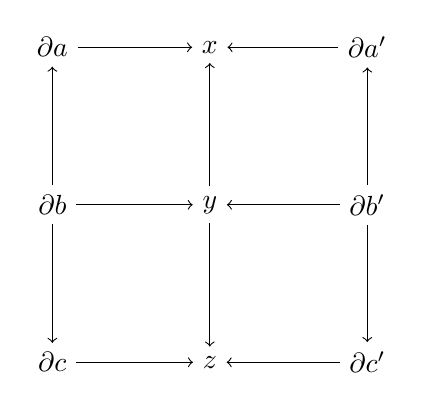
\begin{tikzpicture}
	\node (a) at (-1,1) {$ \partial a $};
	\node (x) at (1,1) {$ x $};
	\node (a') at (3,1) {$ \partial a' $};
	\node (b) at (-1,-1) {$ \partial b $};
	\node (y) at (1,-1) {$ y $};
	\node (b') at (3,-1) {$ \partial b' $};
	\node (c) at (-1,-3) {$ \partial c $};
	\node (z) at (1,-3) {$ z $};
	\node (c') at (3,-3) {$ \partial c' $};
	%
	\draw [->] (a) to (x);
	\draw [->] (a') to (x);
	\draw [->] (b) to (y);
	\draw [->] (b') to (y);
	\draw [->] (c) to (z);
	\draw [->] (c') to (z);
	\draw [->] (b) to (a);
	\draw [->] (b) to (c);
	\draw [->] (y) to (x);
	\draw [->] (y) to (z);
	\draw [->] (b') to (a');
	\draw [->] (b') to (c');
\end{tikzpicture}
\]
If we borrow a perspective from Section \ref{sec:Rewriting}, we can think of an arrow as a rewrite rule as long as $ \OpenOb{\partial} $ is adhesive. From now, we assume that this is the case, which Corollary \ref{thm:OpenObAdhsv} ensures is a reasonable assumption.  It is tempting to rename $ \Sp{\OpenOb{\partial}} $ to something that indicates the arrows are rewrites of open objects.  However, this bicategory is too constrictive.  Yes, it allows us to compose rewrites, but we cannot connect open objects together along their boundary. This was the whole impetus to create open objects.  Because connecting open objects is actually composition in $ \FuncCsp{\partial} $, we want a structure that suitably combines both $ \FuncCsp{\partial} $ and $ \Sp{\OpenOb{\partial}} $.  The natural choice is a double category.  

Some grooming is necessary before we can get an actual double category.  The primary hurdle is ensuring the interchange law holds.  At this point, our framework branches into two paths.  We look at two categories constructed from the information of $ \Sp{\OpenOb{\partial}} $, each serving as a category of arrows for a double category with $ \FuncCsp{\partial} $ as its category of objects.

\begin{df} \label{df:ArrCatMonRwrt}
	There is a preorder with objects those from $ \Sp{\OpenOb{\partial}} $ and we write $ (\partial a \to x \gets \partial a') \leq (\partial c \to x \gets \partial c') $ if there is an arrow in $ \Sp{\OpenOb{\partial}} $ with form
	\[
	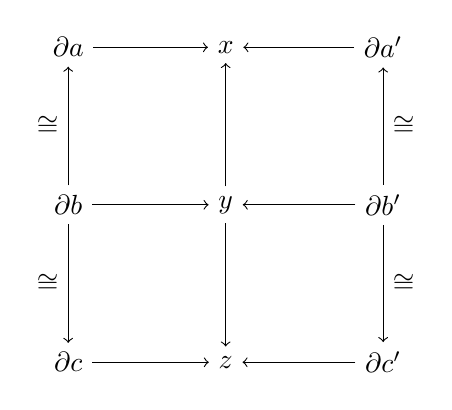
\begin{tikzpicture}
		\node (a) at (-1,1) {$ \partial a $};
		\node (x) at (1,1) {$ x $};
		\node (a') at (3,1) {$ \partial a' $};
		\node (b) at (-1,-1) {$ \partial b $};
		\node (y) at (1,-1) {$ y $};
		\node (b') at (3,-1) {$ \partial b' $};
		\node (c) at (-1,-3) {$ \partial c $};
		\node (z) at (1,-3) {$ z $};
		\node (c') at (3,-3) {$ \partial c' $};
		%
		\draw [->] (a) to (x);
		\draw [->] (a') to (x);
		\draw [->] (b) to (y);
		\draw [->] (b') to (y);
		\draw [->] (c) to (z);
		\draw [->] (c') to (z);
		\draw [->] (b) to node [left] {$ \cong $} (a);
		\draw [->] (b) to node [left] {$ \cong $} (c);
		\draw [->] (y) to (x);
		\draw [->] (y) to (z);
		\draw [->] (b') to node [right] {$ \cong $} (a');
		\draw [->] (b') to node [right] {$ \cong $} (c');
	\end{tikzpicture}
	\]
\end{df}

\begin{df} \label{df:ArrCatRwrt}
	There is a category with objects those from $ \Sp{\OpenOb{\partial}} $ and arrows are isomorphism classes of 1-cells of form
\[
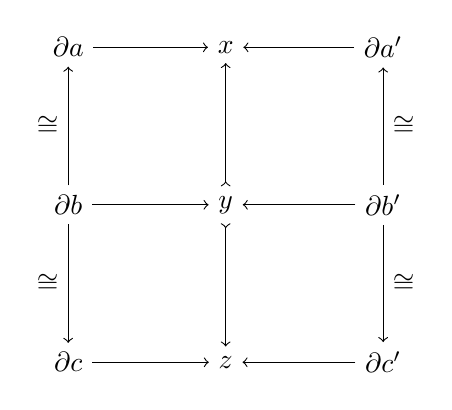
\begin{tikzpicture}
	\node (a) at (-1,1) {$ \partial a $};
	\node (x) at (1,1) {$ x $};
	\node (a') at (3,1) {$ \partial a' $};
	\node (b) at (-1,-1) {$ \partial b $};
	\node (y) at (1,-1) {$ y $};
	\node (b') at (3,-1) {$ \partial b' $};
	\node (c) at (-1,-3) {$ \partial c $};
	\node (z) at (1,-3) {$ z $};
	\node (c') at (3,-3) {$ \partial c' $};
	%
	\draw [->] (a) to (x);
	\draw [->] (a') to (x);
	\draw [->] (b) to (y);
	\draw [->] (b') to (y);
	\draw [->] (c) to (z);
	\draw [->] (c') to (z);
	\draw [->] (b) to node [left] {$ \cong $} (a);
	\draw [->] (b) to node [left] {$ \cong $} (c);
	\draw [>->] (y) to (x);
	\draw [>->] (y) to (z);
	\draw [->] (b') to node [right] {$ \cong $} (a');
	\draw [->] (b') to node [right] {$ \cong $} (c');
\end{tikzpicture}
\]
where the arrows marked ``$ \rightarrowtail $'' are monic. 
\end{df}

{\color{red}\emph{(are these constructions functorial?)}}

%%%%%%%%%%%%%%%%%%%%%%%%%%%%%%%
%%%%%%%%%%%%%%%%%%%%%%%%%%%%%%%
\section{Double categories for rewriting}

Recall the functor $ \core{-} \from \Cat \to \cat{Grpd} $ that sends a category its maximal sub-groupoid.

%%%%%%%%%%%%%%%%%%%
\subsection{Monic spans of cospans}

\emph{(Here is some stuff about the double category of monic spans of cospans.)}

\begin{df}
	Define the double category $ \MMonRewrite{\partial} $ to have $ \core{ \Sp{\A}} $ as its category of objects and the category of arrows is as described in Definition \ref{df:ArrCatMonRwrt}. 
\end{df}

\begin{thm}
	The double category $ \MMonRewrite{\partial} $ is isofibrant.
\end{thm}

\begin{thm}
	If $ \partial \dashv p \from (\A, \otimes_{\A}) \to (\X, \otimes_{\X}) $ is an adjunction of symmetric monoidal categories, then $ \MMonRewrite{\partial} $ is a symmetric monoidal double category via
	\[
	\left( \partial a \to x \gets \partial b \right) \otimes
	\left( \partial c \to y \gets \partial d	\right) \coloneqq
	\partial (a \otimes_{\A} c) \to 
		x \otimes_{\X} y \gets \partial (b \otimes_{\A} d)
	\]
\end{thm}

\begin{thm}
	The globular bicategory $ \MonRewrite{\partial} \coloneqq  \mathcal{H} \left( \MMonRewrite{\partial} \right) $ in the sense of Shulman is symmetric monoidal.  Moreover, if the monoidal products $ \otimes_{\A} $ and $ \otimes_{\X} $ are coproducts, then the symmetric monoidal bicategory $ \MonRewrite{\partial} $ is compact closed.
\end{thm}

\emph{(And now we transition to the double category of spans of cospans.)}

%%%%%%%%%%%%%%%%
\subsection{Spans of cospans}

\emph{(Here is some stuff about the double category of spans of cospans.)}

\begin{df}
	Define the double category $ \RRewrite{\partial} $ to have $ \core{\Sp{\A}} $ as its category of objects and its category of arrows a described in Definition \ref{df:ArrCatRwrt}.
\end{df}

\begin{thm}
	The double category $ \RRewrite{\partial} $ is isofibrant.
\end{thm}

\begin{thm}
	If $ \partial \dashv p \from (\A, \otimes_{\A}) \to (\X, \otimes_{\X}) $ is an adjunction of symmetric monoidal categories, then $ \Rewrite{\partial} $ is a symmetric monoidal double category via
	\[
	\left( \partial a \to x \gets \partial b \right) \otimes
	\left( \partial c \to y \gets \partial d	\right) \coloneqq
	\partial (a \otimes_{\A} c) \to 
	x \otimes_{\X} y \gets \partial (b \otimes_{\A} d)
	\]
\end{thm}

\begin{thm}
	The globular bicategory $ \Rewrite{\partial} \coloneqq  \mathcal{H} \left( \MMonRewrite{\partial} \right) $ in the sense of Shulman is symmetric monoidal.  Moreover, if the monoidal products $ \otimes_{\A} $ and $ \otimes_{\X} $ are coproducts, then the symmetric monoidal bicategory $ \MonRewrite{\partial} $ is compact closed.
\end{thm}

\begin{thm}
	The bicategory $ \Rewrite{\partial} $ is a bicategory of relations in the sense of Carboni and Walters.
\end{thm}
 
 \emph{(some cool stuff abt bicats of rels and how it relates to networks.)}
 
 %%%%%%%%%%%%%%%%%%%%%%%%%%%%
 \section{Rewriting open objects}
 
 \emph{(Exposit on the two rewrite bicategories and their relation to network rewriting.  Bring languages into it.)}
 
Same adjunction $ \partial \dashv p \from \A \to \X $ between topoi.
 
\begin{df}
	Fix a grammar $ \Gamma $ in the topos $ \OpenOb{\partial} $. Hence, it is a set of morphisms in $ \Sp{\OpenOb{\partial}} $.  The generated  language $ \mathcal{L}(\Gamma) $ is a sub-bicategory of $ \Sp{\OpenOb{\partial}} $. 
\end{df}

\begin{thm}
	Suppose each element from a grammar $ \Gamma $ in $ \OpenOb{\partial} $ is of the form 
	\[
	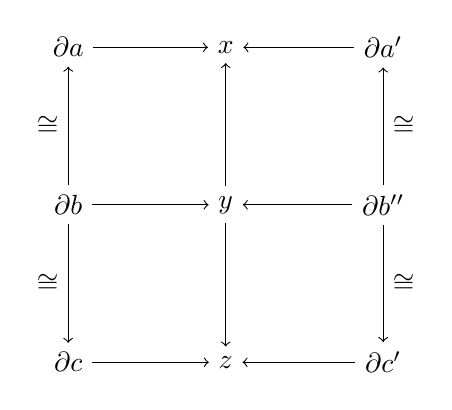
\begin{tikzpicture}
		\node (a) at (-1,1) {$ \partial a $};
		\node (x) at (1,1) {$ x $};
		\node (a') at (3,1) {$ \partial a' $};
		\node (b) at (-1,-1) {$ \partial b $};
		\node (y) at (1,-1) {$ y $};
		\node (b') at (3,-1) {$ \partial b'' $};
		\node (c) at (-1,-3) {$ \partial c $};
		\node (z) at (1,-3) {$ z $};
		\node (c') at (3,-3) {$ \partial c' $};
		%
		\draw [->] (a) to (x);
		\draw [->] (a') to (x);
		\draw [->] (b) to (y);
		\draw [->] (b') to (y);
		\draw [->] (c) to (z);
		\draw [->] (c') to (z);
		\draw [->] (b) to node [left] {$ \cong $} (a);
		\draw [->] (b) to node [left] {$ \cong $} (c);
		\draw [->] (y) to (x);
		\draw [->] (y) to (z);
		\draw [->] (b') to node [right] {$ \cong $} (a');
		\draw [->] (b') to node [right] {$ \cong $} (c');
	\end{tikzpicture}
	\]
	then $ \Gamma $ generates a sub-double category of $ \RRewrite{\partial} $.   The recipe is get the language $ \mathcal{L}(\Gamma)  \subseteq \Sp{\OpenOb{\partial}} $. Form the category as described in Definition \ref{df:ArrCatRwrt} from $ \mathcal{L}(\Gamma) $. Pair this, as an arrow category, with the object category $ \core{\Sp{\A}} $.  
\end{thm}

\begin{thm}
	Suppose each element from a grammar $ \Gamma $ in $ \OpenOb{\partial} $ is of the form 
	\[
	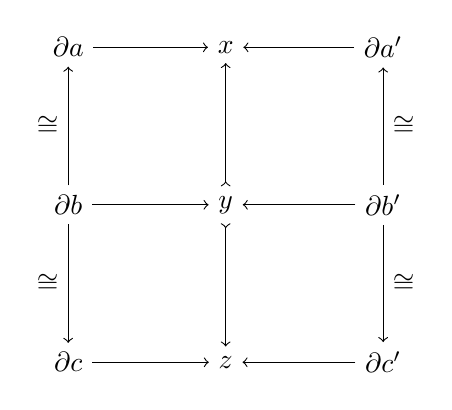
\begin{tikzpicture}
	\node (a) at (-1,1) {$ \partial a $};
	\node (x) at (1,1) {$ x $};
	\node (a') at (3,1) {$ \partial a' $};
	\node (b) at (-1,-1) {$ \partial b $};
	\node (y) at (1,-1) {$ y $};
	\node (b') at (3,-1) {$ \partial b' $};
	\node (c) at (-1,-3) {$ \partial c $};
	\node (z) at (1,-3) {$ z $};
	\node (c') at (3,-3) {$ \partial c' $};
	%
	\draw [->] (a) to (x);
	\draw [->] (a') to (x);
	\draw [->] (b) to (y);
	\draw [->] (b') to (y);
	\draw [->] (c) to (z);
	\draw [->] (c') to (z);
	\draw [->] (b) to node [left] {$ \cong $} (a);
	\draw [->] (b) to node [left] {$ \cong $} (c);
	\draw [>->] (y) to (x);
	\draw [>->] (y) to (z);
	\draw [->] (b') to node [right] {$ \cong $} (a');
	\draw [->] (b') to node [right] {$ \cong $} (c');
	\end{tikzpicture}
	\]
	then $ \Gamma $ generates a sub-double category $ \langle \langle \Gamma \rangle \rangle $ of $ \MMonRewrite{\partial} $.  The recipe is get the language $ \mathcal{L}(\Gamma)  \subseteq \Sp{\OpenOb{\partial}} $. Form the category as described in Definition \ref{df:ArrCatMonRwrt} from $ \mathcal{L}(\Gamma) $. Pair this, as an arrow category, with the object category $ \core{\Sp{\A}} $.
\end{thm}

{\color{red}\emph{(Can we do this functorially? Define a bicategory with pairs $ (\A , \Gamma) $ and adhesive category and the bicategory of double categories, then the above construction is a functor from the former to the latter?)}}

\begin{thm}
	If $ \Gamma $ has only elements of the form 
	\[
	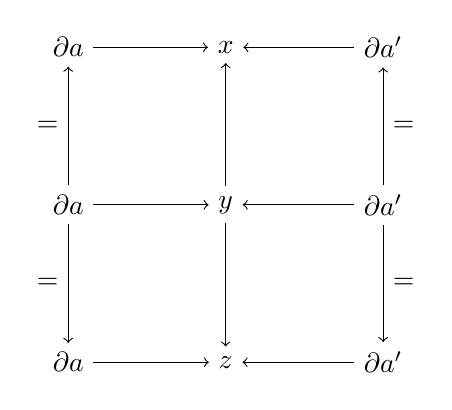
\begin{tikzpicture}
		\node (a) at (-1,1) {$ \partial a $};
		\node (x) at (1,1) {$ x $};
		\node (a') at (3,1) {$ \partial a' $};
		\node (b) at (-1,-1) {$ \partial a $};
		\node (y) at (1,-1) {$ y $};
		\node (b') at (3,-1) {$ \partial a' $};
		\node (c) at (-1,-3) {$ \partial a $};
		\node (z) at (1,-3) {$ z $};
		\node (c') at (3,-3) {$ \partial a' $};
		%
		\draw [->] (a) to (x);
		\draw [->] (a') to (x);
		\draw [->] (b) to (y);
		\draw [->] (b') to (y);
		\draw [->] (c) to (z);
		\draw [->] (c') to (z);
		\draw [->] (b) to node [left] {$ = $} (a);
		\draw [->] (b) to node [left] {$ = $} (c);
		\draw [->] (y) to (x);
		\draw [->] (y) to (z);
		\draw [->] (b') to node [right] {$ = $} (a');
		\draw [->] (b') to node [right] {$ = $} (c');
	\end{tikzpicture}
	\]
	then $ \Gamma $ generates a sub-bicategory of $ \Rewrite{\partial} $.  This sub-bicategory corresponds to the sub-bicategory of $ \Rewrite{\partial} $ obtained by passing the construction through $ \RRewrite{\partial} $ first, then applying $ \mathcal{H}(-) $.  
\end{thm}

\begin{thm}
	Same as above with monics thrown in.
\end{thm}

%%%%%%%%%%%%%%%%%%%%%%%%%%%%%%
%%%%%%%%%%%%%%%%%%%%%%%%%%%%%%
\section{Local Church-Rosser \& concurrency}

{\color{red}\emph{Do these hold in the grammar generated bicategories?}}

%%%%%%%%%%%%%%%%%%%%%%%%%%%%%%
%%%%%%%%%%%%%%%%%%%%%%%%%%%%%%
\section{Examples}

{\color{red}\emph{string diagrams for Frobenius monoids // linguistics ex?}}



\end{document}